\section{Rankingi}
Ranking mobilny bazuje na około 973 tys. pomiarów w sieciach 3G, 4G LTE i 5G. Średnia prędkość pobierania Plusa w III kwartale wyniosła blisko 50 Mb/s.

W 3. kwartale wykonano 83 tysiące testów w technologii 5G, a liczba ta stale rośnie, co świadczy o coraz większej popularności tej technologii. Najszybszym operatorem był Plus ze średnim wynikiem pobierania prędkości 134 Mb/s.

\begin{figure}[!htb]
    \centering
    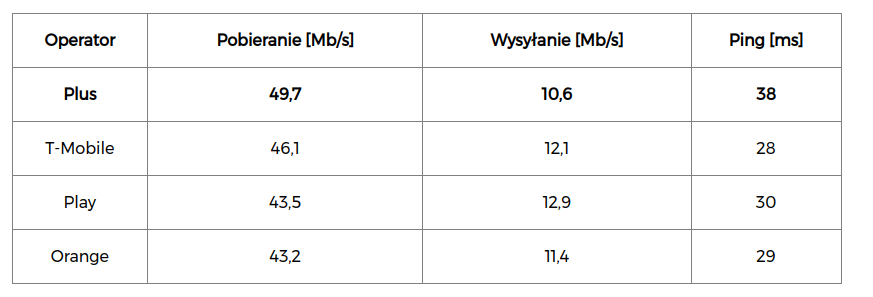
\includegraphics[width=0.7\textwidth]{r1}
    \caption{Ranking internetu mobilnego w 3. kwartale 2023}
\end{figure}


\begin{figure}[!htb]
    \centering
    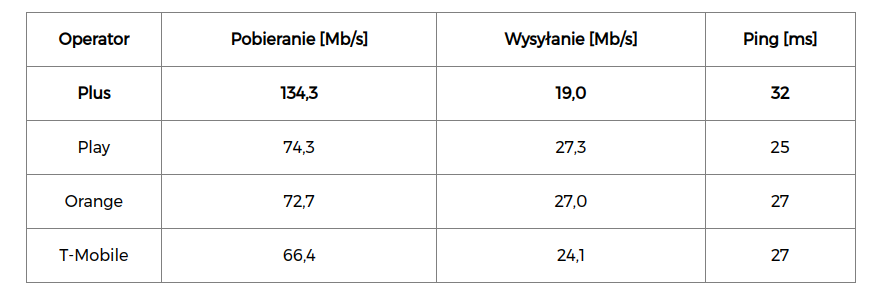
\includegraphics[width=0.7\textwidth]{r2}
    \caption{Ranking 5G w 3. kwartale 2023}
\end{figure}
